\documentclass{ximera}

\usepackage{microtype}
\usepackage{tikz}
\usepackage{tkz-euclide}
\usetkzobj{all}
\tikzstyle geometryDiagrams=[ultra thick,color=blue!50!black]

\renewcommand{\epsilon}{\varepsilon}



\title{Central projection}
\begin{document}
\begin{abstract}
Here we start to develop a model for our geometry.
\end{abstract}
\maketitle



\section{Central projection coordinates}

Let's project $K$-geometry,
\[
1=K\left(x^{2}+y^{2}\right)+z^{2} 
\]
onto the plane $z=1$ using the origin $O=(0,0,0)$ as the center of
projection:
\[
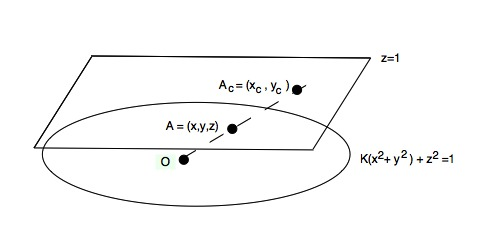
\includegraphics[width=3in]{MXAJBZ0K.jpg}
\qquad
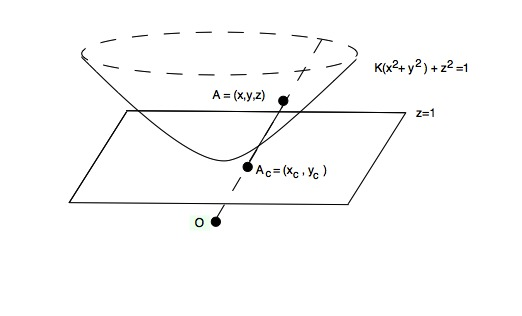
\includegraphics[width=3in]{MXAJBZ0L.jpg}
\]
Let's look at this from a different vantage point, say with our eye parallel to the plane $z=1$.
\[
\text{IMAGE: side view with $r$ labeled}
\]
Note, we are only projecting the top of the surface
\[
1=K\left(x^{2}+y^{2}\right)+z^{2} 
\]
onto the plane $z=1$. So when $K>0$, this is the ``Northern hemisphere'' of
the sphere, when $K<0$, this is the upper hyperboloid, and when $K=0$,
this is the plane $z=1$.

\begin{problem}
  What range of values could $r$ take when $K>0?$?
  \begin{freeResponse}
    In this case, $r\in (0,1)$.
  \end{freeResponse}
\end{problem}

\begin{problem}
  What range of values could $r$ take when $K<0?$?
  \begin{freeResponse}
    In this case, $r\in(1,\infty)$.
  \end{freeResponse}
\end{problem}

\begin{problem}
  What range of values could $r$ take when $K=0?$?
  \begin{freeResponse}
    In this case
    \[
    1=K\left(x^{2}+y^{2}\right)+z^{2} 
    \]
    is the plane $z = 1$, hence $r=1$.
  \end{freeResponse}
\end{problem}

\begin{problem}
  Letting $(x_c,y_c,1)$ be the image of the $K$-geometry points
  $(x,y,z)$ in the plane $z=1$, use facts about similar triangles to
  explain why
  \[
  r\cdot(x_{c},y_{c},1)=(x,y,z).
  \]
\end{problem}


\begin{problem}
  For the projection of the set $1=K\left(x^{2}+y^{2}\right)+z^{2}$
  onto the $z=1$ plane with center of projection $O$, write
  $(x_{c},y_{c})$ as a function of $(x,y,z)$.
  \begin{freeResponse}
    We know that
    \[
    r\cdot(x_{c},y_{c},1)=(x,y,z),
    \]
    hence $r=z$, and we may now write
    \begin{align*}
      x_{c} &=x/z,\\
      y_{c} &=y/z.
    \end{align*}
  \end{freeResponse}
\end{problem}

\begin{problem}
  For the projection of the set $1=K\left(x^{2}+y^{2}\right)+z^{2} $
  onto the $z=1$ plane with center of projection $O$, write $(x,y,z)$
  as a function of $(x_{c},y_{c})$.
  \begin{freeResponse}
    This is slightly more complex than the previous problem; however,
    we will begin the same way. We know that
    \[
    r\cdot(x_{c},y_{c},1)=(x,y,z),
    \]
    hence $r=z$, and we may now write
    \begin{align*}
      x &= x_c\cdot z,\\
      y &= y_c\cdot z,\\
      z &= z.
    \end{align*}
    Now our task is to write $z$ in terms of $x_c$ and $y_c$. Using our assignments above, write
    \begin{align*}
      1 &= K\left(x^2 + y^2\right) + z^2\\
      1 &= K\left((x_c\cdot z)^2 + (y_c\cdot z)^2\right) + z^2\\
      1 &= \left(K\left(x_c^2 + y_c^2\right)+1\right)z^2,
    \end{align*}
    and so
    \[
    z = \frac{1}{\sqrt{K\left(x_c^2 + y_c^2\right)+1}}.
    \]
    Hence
    \begin{align*}
      x &= \frac{x_c}{\sqrt{K\left(x_c^2 + y_c^2\right)+1}},\\
      y &= \frac{y_c}{\sqrt{K\left(x_c^2 + y_c^2\right)+1}},\\
      z &= \frac{1}{\sqrt{K\left(x_c^2 + y_c^2\right)+1}}.\\
    \end{align*}
  \end{freeResponse}
\end{problem}






\section{Central projection dot product}

Like we have done before, now we want to be able to find a dot product
that will allow us to compute lengths in central prjojection
coordinates that will agree with the $K$-dot product, and hence the
euclidean dot product.


\begin{problem}
Suppose we have a curve $X$ in $K$-warped space that is a function of
a curve $X_c$ in the plane $z=1$ space. So
\[
X_c(t) = \left( x_c(t),y_c(t)\right)
\]
and
\[
X(t) = 
\begin{cases}
  x(x_c(t),y_c(t)),\\
  y(x_c(t),y_c(t)),\\
  z(x_c(t),y_c(t)).
\end{cases}
\]
Use the chain rule to compute
\[
\dd[x]{t}, \qquad \dd[y]{t}, \qquad \dd[z]{t},
\]
in terms of $\dd[x_c]{t}$, $\dd[y_c]{t}$, $\pp[x]{x_c}$,
$\pp[y]{x_c}$, $\pp[z]{x_c}$, $\pp[x]{y_c}$, $\pp[y]{y_c}$,
and $\pp[z]{y_c}$.
  \begin{hint}
  Simply write down the answer from a previous problem with some minor
  changes.
  \end{hint}
  \begin{freeResponse}
  Write
  \begin{align*}
    \dd[x]{t} &= \left(\pp[x]{x_c},\pp[x]{y_c}\right)\bullet\left(\dd[x_c]{t},\dd[y_c]{t}\right) = \pp[x]{x_c}\cdot\dd[x_c]{t}+\pp[x]{y_c}\cdot\dd[y_c]{t}, \\
    \dd[y]{t} &= \left(\pp[y]{x_c},\pp[y]{y_c}\right)\bullet\left(\dd[x_c]{t},\dd[y_c]{t}\right) = \pp[y]{x_c}\cdot\dd[x_c]{t}+\pp[y]{y_c}\cdot\dd[y_c]{t}, \\
    \dd[z]{t} &= \left(\pp[z]{x_c},\pp[z]{y_c}\right)\bullet\left(\dd[x_c]{t},\dd[y_c]{t}\right) = \pp[z]{x_c}\cdot\dd[x_c]{t}+\pp[z]{y_c}\cdot\dd[y_c]{t}.  
  \end{align*}
\end{freeResponse}
\end{problem}




\begin{problem}
  With the same setting as in the previous problem, rewrite the result
  of your computation in matrix notation to find $D_c$
  such that
\[
\begin{bmatrix}
\dd[x]{t} & \dd[y]{t} & \dd[z]{t}
\end{bmatrix}
=
\begin{bmatrix}
\frac{dx_c}{dt} & \frac{dy_c}{dt}
\end{bmatrix}\cdot D_c.
\]
\begin{hint}
  Simply write down the answer from a previous problem with some minor
  changes.
\end{hint}
\begin{freeResponse}
  \[
  D_c =
  \begin{bmatrix}
    \pp[x]{x_c} & \pp[y]{x_c} & \pp[z]{x_c} \\
    \pp[x]{y_c}   & \pp[y]{y_c}   & \pp[z]{y_c}
  \end{bmatrix}.
  \]
\end{freeResponse}
\end{problem}





\begin{problem}
  Now find $P_c$ in terms of $K$, $\pp[x]{x_c}$, $\pp[y]{x_c}$,
  $\pp[z]{x_c}$, $\pp[x]{y_c}$, $\pp[y]{y_c}$, and $\pp[z]{y_c}$
  such that
  \[
  \left(\dd[x]{t}, \dd[y]{t}, \dd[z]{t}\right)\bullet_K
  \left(\dd[x]{t}, \dd[y]{t}, \dd[z]{t}\right)
  =
  \begin{bmatrix}
    \dd[x_c]{t} &  \dd[y_c]{t}
  \end{bmatrix}
  \cdot P_c
  \cdot
  \begin{bmatrix}
    \dd[x_c]{t} \\  \dd[y_c]{t}
  \end{bmatrix}.
  \]
  \begin{hint}
  Simply write down the answer from a previous problem with some minor
  changes.
  \end{hint}
  \begin{freeResponse}
    Working from the $K$-dot product, we need that
    \begin{align*}
    \left(\dd[x]{t}, \dd[y]{t}, \dd[z]{t}\right)\bullet_K
    \left(\dd[x]{t}, \dd[y]{t}, \dd[z]{t}\right)
    &=
    \begin{bmatrix}
      \dd[x]{t} & \dd[y]{t} & \dd[z]{t}
    \end{bmatrix}
    \begin{bmatrix}
      1 & 0 & 0\\
      0 & 1 & 0\\
      0 & 0 & K^{-1}
    \end{bmatrix}
    \begin{bmatrix}
      \dd[x]{t} \\ \dd[y]{t} \\ \dd[z]{t}
    \end{bmatrix}\\
    &=
    \begin{bmatrix}
      \frac{dx_c}{dt} & \frac{dy_c}{dt}
    \end{bmatrix}\cdot D_{c}\cdot
    \begin{bmatrix}
      1 & 0 & 0\\
      0 & 1 & 0\\
    0 & 0 & K^{-1}
    \end{bmatrix}
    \cdot
    \left(
    \begin{bmatrix}
      \frac{dx_c}{dt} & \frac{dy_c}{dt}
    \end{bmatrix}\cdot D_{c}
    \right)^\transpose\\
    &=
    \begin{bmatrix}
      \frac{dx_c}{dt} & \frac{dy_c}{dt}
    \end{bmatrix}\cdot D_{c}\cdot
    \begin{bmatrix}
      1 & 0 & 0\\
      0 & 1 & 0\\
    0 & 0 & K^{-1}
    \end{bmatrix}
    \cdot
    D_{c}^\transpose
    \cdot \begin{bmatrix}
      \frac{dx_c}{dt} \\ \frac{dy_c}{dt}
    \end{bmatrix}.
  \end{align*}
    Hence
    \begin{align*}
      P_c &=
      \begin{bmatrix}
        \pp[x]{x_c} & \pp[y]{x_c} & \pp[z]{x_c} \\
        \pp[x]{y_c} & \pp[y]{y_c} & \pp[z]{y_c}
      \end{bmatrix}
      \begin{bmatrix}
        1 & 0 & 0\\
        0 & 1 & 0\\
        0 & 0 & K^{-1}
      \end{bmatrix}
      \begin{bmatrix}
        \pp[x]{x_c} & \pp[x]{y_c}\\ 
        \pp[y]{x_c} & \pp[y]{y_c}\\
        \pp[z]{x_c} & \pp[z]{y_c}
      \end{bmatrix}\\
      &=
      \begin{bmatrix}
        \left(\pp[x]{x_c}\right)^2 + \left(\pp[y]{x_c}\right)^2 + \left(\pp[z]{x_c}\right)^2K^{-1} & \pp[x]{x_c}\pp[x]{y_c} + \pp[y]{x_c}\pp[y]{y_c} + \pp[z]{x_c}\pp[z]{y_c} K^{-1}\\
        \pp[x]{x_c}\pp[x]{y_c} + \pp[y]{x_c}\pp[y]{y_c} + \pp[z]{x_c}\pp[z]{y_c} K^{-1}       & \left(\pp[x]{y_c}\right)^2 + \left(\pp[y]{y_c}\right)^2 + \left(\pp[z]{y_c}\right)^2K^{-1}
      \end{bmatrix}.
    \end{align*}
  \end{freeResponse}
\end{problem}


\begin{problem}
  Set
  \begin{align*}
    x(x_c,y_c) &=|K|^{-1/2}\cdot \sinh x_c\cdot \cos y_c,\\
    y(x_c,y_c) &=|K|^{-1/2}\cdot \sinh x_c\cdot \sin y_c,\\
    z(x_c,y_c) &=\cosh\sigma,
  \end{align*}
  and show that $P_c$ from the problem above is
  \[
P_c = \begin{bmatrix}
r^{2}\left(  1-Kx_{c}^{2}r^2\right)  & -Kx_{c}y_{c}r^4\\
-Kx_{c}y_{c}r^4 & r^{2}\left(  1-Ky_{c}^{2}r^2\right)
\end{bmatrix}.
\]
\begin{hint}
  To compute the partial derivatives, work in the following way:
  \begin{enumerate}
  \item Recall $x = r\cdot x_c$.
  \item Note that $\pp[x]{x_c} = r + x_c \cdot \pp[r]{x_c}$.
    \item Express the partial derivative in terms of $r$, $K$, $x_c$,
      and $y_c$.
  \end{enumerate}
\end{hint}
\begin{hint}
  When simpliying, combine the terms with the highest degree of $r$
  and note that
  \[
  r^{-2} = K\left(x_c^2 + y_c^2\right) + 1.
  \]
\end{hint}
\begin{freeResponse}
  Write
  \begin{align*}
    \pp[x]{x_c} &= r  + x_c \cdot \pp[r]{x_c}\\
    &= r + x_c \cdot \pp{x_c} \left(K\left(x_c^2 + y_c^2\right)+1\right)^{-1/2}\\
    &= r + x_c \cdot (-1/2)\left(K\left(x_c^2 + y_c^2\right)+1\right)^{-3/2}(2Kx_c)\\
    &= r -Kx_c^2 r^3.
  \end{align*}
  Similarly,
    \begin{align*}
    \pp[y]{x_c} &= y_c \cdot \pp[r]{x_c}\\
    &= y_c \cdot \pp{x_c} \left(K\left(x_c^2 + y_c^2\right)+1\right)^{-1/2}\\
    &= y_c \cdot (-1/2)\left(K\left(x_c^2 + y_c^2\right)+1\right)^{-3/2}(2Kx_c)\\
    &= -Kx_cy_c r^3.
    \end{align*}
   Finally, 
    \begin{align*}
    \pp[z]{x_c} &= \pp[r]{x_c}\\
    &= \pp{x_c}\left(K\left(x_c^2 + y_c^2\right)+1\right)^{-1/2}\\
    &= (-1/2)\left(K\left(x_c^2 + y_c^2\right)+1\right)^{-3/2}(2Kx_c)\\
    &= -Kx_c r^3.
    \end{align*}
    Now with entirely similar computations, we see
    \begin{align*}
      \pp[x]{y_c} &= -Kx_cy_c r^3,\\
      \pp[y]{y_c} &= r - Ky_c^2 r^3,\\
      \pp[z]{y_c} &= -Ky_c r^3.
    \end{align*}


    
    Now we see $\left(\pp[x]{x_c}\right)^2 + \left(\pp[y]{x_c}\right)^2 + \left(\pp[z]{x_c}\right)^2K^{-1}$
    \begin{align*}
      &= \left(r -Kx_c^2 r^3\right)^2 + \left(-Kx_cy_c r^3\right)^2 + \left(-Kx_c r^3\right)^2K^{-1}\\
      &= r^2 - 2Kx_c^2r^4 + K^2x_c^4 r^6+ K^2x_c^2y_c^2r^6 + Kx_c^2r^6\\
      &= r^2 - 2Kx_c^2r^4 + Kx_c^2r^6\left(Kx_c^2 + Ky_c^2 + 1\right)\\
      &= r^2 - 2Kx_c^2r^4 + Kx_c^2r^6\left(K\left(x_c^2 + y_c^2\right) + 1\right)\\
      &= r^2 - 2Kx_c^2r^4 + Kx_c^2r^6 r^{-2}\\
      &= r^2 - 2Kx_c^2r^4 + Kx_c^2r^4\\
      &= r^2 - Kx_c^2r^4\\
      &= r^2(1 - Kx_c^2r^2).\\
    \end{align*}
    
    That $\pp[x]{x_c}\pp[x]{y_c} + \pp[y]{x_c}\pp[y]{y_c} + \pp[z]{x_c}\pp[z]{y_c} K^{-1}$
    \begin{align*}
      &=\left(r -Kx_c^2 r^3\right)\left(-Kx_cy_c r^3\right) + \left(-Kx_cy_c r^3\right)\left(r - Ky_c^2 r^3\right) + \left(-Kx_c r^3\right)\left(-Ky_c r^3\right)K^{-1}\\
      &= -Kx_cy_cr^4+K^2x_c^3y_cr^6-Kx_cy_cr^4+K^2x_cy_c^3r^6+Kx_cy_cr^6\\
      &= K^2x_c^3y_cr^6+K^2x_cy_c^3r^6+Kx_cy_cr^6 -2Kx_cy_cr^4\\
      &= Kx_cy_cr^6\left(K\left(x_c^2 + y_c^2\right) + 1\right)-2Kx_cy_cr^4\\
      &= Kx_cy_cr^6r^{-2} -2Kx_cy_cr^4\\
      &= Kx_cy_cr^4 -2Kx_cy_cr^4\\
      &= -Kx_cy_cr^4.
    \end{align*}
    With entirely analogus computations, we see that 
    \[
     P_c =
     \begin{bmatrix}
       r^{2}\left( 1-Kx_{c}^{2}r^2\right) & -Kx_{c}y_{c}r^4\\
       -Kx_{c}y_{c}r^4 & r^{2}\left(1-Ky_{c}^{2}r^2\right)
     \end{bmatrix}.
     \]
  \end{freeResponse}
\end{problem}


\begin{definition}
  Let $V_c$ be a vector in $(x_c,y_c)$-coordinates. Define
  \[
  V_c \bullet_c V_c = V_c \cdot P_c \cdot V_c^\transpose.
  \]
\end{definition}

\begin{warning}
  Note, we have only defined $V_c\bullet_c W_c$ for the (very) special
  case of when $V_c = W_c$. However, this will be enough for our
  purposes.
\end{warning}











\section{Rigid motions in central projection coordinates}

Suppose now we have a $K$-rigid motion
\[
\left(  \underline{x},\underline{y},\underline{z}\right)  =\left(
x,y,z\right)  \cdot M
\]
of $K$-geometry, given by a $K$-orthogonal matrix%
\[
M=\begin{bmatrix}
m_{11} & m_{12} & m_{13}\\
m_{21} & m_{22} & m_{23}\\
m_{31} & m_{32} & m_{33}
\end{bmatrix}.
\]
Let's convert this $K$-rigid motion to a rigid motion in central
projection coordinates. This new rigid motion will not necessarily be
a mapping defined by a matrix, so we'll have to use some new notation.


\begin{image}
\begin{tikzpicture}
  \node (xyz) {$\begin{bmatrix}x & y & z\end{bmatrix}\in\mathbb{R}^3$};
  \node (xyzBar) [node distance=2cm,below of=xyz] {$\begin{bmatrix}\underline{x} & \underline{y} & \underline{z}\end{bmatrix}$};
  \node (xcyc1) [node distance=4cm,right of=xyz] {$(x_c,y_c,1)\in\mathbb{R}^2\times\{1\}$};
  \node (xcyc1Bar) [node distance=4cm,right of=xyzBar] {$(\underline{x_c},\underline{y_c},1)$};
  \node (xcyc) [node distance=4cm,right of=xcyc1] {$(x_c,y_c)\in\mathbb{R}^2$};
  \node (xcycBar) [node distance=4cm,right of=xcyc1Bar] {$(\underline{x_c},\underline{y_c})$};
  \draw[->] (xcyc1) to node[above] {$\cdot r$} (xyz);
  \draw[->] (xcyc1Bar) to node [above] {$\cdot\underline{r}$} (xyzBar);
  \draw[left hook->] (xcyc) to (xcyc1);
  \draw[left hook->] (xcycBar) to (xcyc1Bar);

  \draw[->] (xyz) to node[right] {$\cdot M$} (xyzBar);
  \draw[->] (xcyc1) to node[right] {$\mu_{c'}=?$} (xcyc1Bar);
  \draw[->] (xcyc) to node[right] {$\mu_{c}=?$} (xcycBar);
\end{tikzpicture}
\end{image}

\begin{problem}
  Using the diagram above, explain why
  \begin{align*}
(\underline{x_{c}},\underline{y_{c}})  &= \mu_{c}(x_{c},y_{c}) \\
  & =\left(\frac{m_{11}x_{c}+m_{21}y_{c}+m_{31}}{m_{13}x_{c}+m_{23}y_{c}+m_{33}},
  \frac{m_{12}x_{c}+m_{22}y_{c}+m_{32}}{m_{13}x_{c}+m_{23}y_{c}+m_{33}
}\right).
  \end{align*}
  \begin{freeResponse}
    Let's follow this diagram around, starting at the right-most
    corner. We want to start with $(x_c,y_c)$ and end with
    $(\underline{x_c},\underline{y_c} = \mu_c(x_c,y_c)$. Since $\R^2$
    embeeds canonically into $\R^2\times\{1\}$, we move to the
    upper-middle position almost immedately. Now, via multiplication
    by $r$, $(x_c,y_c,1)$ maps to $(x,y,z)$. From here we may use
    matrix multiplication
    \[
    \begin{bmatrix}
      \underline{x} & \underline{y} & \underline{z}
    \end{bmatrix}
    =
    \begin{bmatrix}
    x & y & z
    \end{bmatrix}
    \cdot\begin{bmatrix}
    m_{11} & m_{12} & m_{13}\\
    m_{21} & m_{22} & m_{23}\\
    m_{31} & m_{32} & m_{33}
    \end{bmatrix}.
    \]
    Expanded out, this is
    \[
    \begin{bmatrix}
      m_{11}x+m_{21}y+m_{31}z & m_{12}x+m_{22}y+m_{32}z & 
      m_{13}x+m_{23}y+m_{33}z
    \end{bmatrix}.
    \]
    We are now at the bottom left-hand corner of our diagram. To move
    to the lower position, we multiply by $\underline{r}^{-1}$, which
    is equivalent to dividing by $\underline{z}$. Hence our element
    becomes
     \[
    \begin{bmatrix}
      \frac{m_{11}x+m_{21}y+m_{31}z}{m_{13}x+m_{23}y+m_{33}z} &
      \frac{m_{12}x+m_{22}y+m_{32}z}{m_{13}x+m_{23}y+m_{33}z} & 1
    \end{bmatrix}.
    \]
    To write this in terms of $x_c$ and $y_c$, we must divide each
    numerator and denominator by $z$
    \[
    \begin{bmatrix}
      \frac{m_{11}(x/z)+m_{21}(y/z)+m_{31}}{m_{13}(x/z)+m_{23}(y/z)+m_{33}}
      &
      \frac{m_{12}(x/z)+m_{22}(y/z)+m_{32}}{m_{13}(x/z)+m_{23}(y/z)+m_{33}}
      & 1
    \end{bmatrix}.
    \]
    Now since $x/z = x_c$ and $y/z =y_c$, we may pull this back to
    $\R^2$ in the lower left-hand corner and write
    \[
    \mu_c(x_c,y_c) = \left(
    \frac{m_{11}x_c+m_{21}y_c+m_{31}}{m_{13}x_c+m_{23}y_c+m_{33}},
    \frac{m_{12}x_c+m_{22}y_c+m_{32}}{m_{13}x_c+m_{23}y_c+m_{33}}
    \right).
    \]
  \end{freeResponse}
\end{problem}


\section{Length and angle in central projection coordinates}

\begin{problem}
\label{33}For the $K$-geometry coordinates%
\[
X=\left(  x,y,z\right)
\]
use the formulas you derived in a previous problem to calculate%
\[
dX=\left(  \frac{\partial X}{\partial x_{c}}\right)  dx_{c}+\left(
\frac{\partial X}{\partial y_{c}}\right)  dy_{c}%
\]
That is, calculate the $2\times3$ matrix%
\[
D_{c}=\begin{bmatrix}
\frac{\partial x}{\partial x_{c}} & \frac{\partial y}{\partial x_{c}} &
\frac{\partial z}{\partial x_{c}}\\
\frac{\partial x}{\partial y_{c}} & \frac{\partial y}{\partial y_{c}} &
\frac{\partial z}{\partial y_{c}}%
\end{bmatrix} =\begin{bmatrix}
\left(  \frac{\partial X}{\partial x_{c}}\right) \\
\left(  \frac{\partial X}{\partial y_{c}}\right)
\end{bmatrix} .
\]
\begin{hint}
Use logarithmic differentiation:%
\begin{align*}
dx  &  =d\left(  rx_{c}\right)  =x_{c}dr+rdx_{c}\\
r^{-1}dx  &  =x_{c}d\ln\left(  r\right)  +dx_{c}%
\end{align*}
and similarly for $y$ and $z$ since it is easier to compute $r^{-1}\left(
\frac{dx}{dt},\frac{dy}{dt},\frac{dz}{dt}\right)  $ than $\left(  \frac
{dx}{dt},\frac{dy}{dt},\frac{dz}{dt}\right)  $. Next use that%
\begin{align*}
2d\ln\left(  r\right)   &  =d\ln\left(  r^{2}\right)
=-d\ln\left(  K\left(  x_{c}^{2}+y_{c}^{2}\right)  +1\right) \\
&  =-\frac{1}{K\left(  x_{c}^{2}+y_{c}^{2}\right)  +1}d\left(  K\left(
x_{c}^{2}+y_{c}^{2}\right)  +1\right) \\
&  =-r^{2}K\left(  2x_{c}dx_{c}+2y_{c}dy_{c}\right)  .
\end{align*}
\end{hint}
\end{problem}

\begin{problem}
\label{prev}Now suppose we have a path,%
\[
\left(  x_{c}\left(  t\right)  ,y_{c}\left(  t\right)  \right)  ,\;a\leq t\leq
b
\]
in the $\left(  x_{c},y_{c}\right)  $-plane, that is, in the central
projection plane%
\[
\left(  x_{c},y_{c},1\right)  .
\]
Use the formula you derived in a previous problem to write the
corresponding path%
\[
x\left(  x_{c}\left(  t\right)  ,y_{c}\left(  t\right)  \right)  ,y\left(
x_{c}\left(  t\right)  ,y_{c}\left(  t\right)  \right)  ,z\left(  x_{c}\left(
t\right)  ,y_{c}\left(  t\right)  \right)
\]
in the $K$-geometry space of $\left(  x,y,z\right)  $ such that $K\left(
x^{2}+y^{2}\right)  +z^{2}=1$.
\end{problem}

\begin{problem}
For the path $\left( x\left( t\right) ,y\left( t\right) ,z\left(
t\right) \right) $ in a previous problem lying on the set
$1=K\left(x^{2}+y^{2}\right)+z^{2} $, use the Chain Rule from calculus
of several variables to compute%
\[
\left(  \frac{dx}{dt},\frac{dy}{dt},\frac{dz}{dt}\right)  =\left(
\frac{dx_{c}\left(  t\right)  }{dt},\frac{dy_{c}\left(  t\right)  }%
{dt}\right)  \cdot D_{c}.
\]

\end{problem}

This last Problem allows us to do something very nice. Namely now, not only
can we use the coordinates $\left(  x_{c},y_{c}\right)  $ for our geometry but
we can also compute the $K$-dot product in terms of these coordinates. By the
Chain Rule from calculus of several variables%
\[
\left(  \frac{dx}{dt},\frac{dy}{dt},\frac{dz}{dt}\right)  =\left(
\frac{dx_{c}}{dt},\frac{dy_{c}}{dt}\right)  \cdot D_{c}.
\]
So%
\begin{align*}
\left(  \frac{dx}{dt},\frac{dy}{dt},\frac{dz}{dt}\right)  \bullet_{K}\left(
\frac{dx}{dt},\frac{dy}{dt},\frac{dz}{dt}\right)   &  =\begin{bmatrix}
\frac{dx}{dt} & \frac{dy}{dt} & \frac{dz}{dt}%
\end{bmatrix} \begin{bmatrix}
1 & 0 & 0\\
0 & 1 & 0\\
0 & 0 & K^{-1}%
\end{bmatrix} \begin{bmatrix}
\frac{dx}{dt}\\
\frac{dy}{dt}\\
\frac{dz}{dt}%
\end{bmatrix}\\
&  =
\begin{bmatrix}
\frac{dx_{c}}{dt} & \frac{dy_{c}}{dt}%
\end{bmatrix} \cdot D_{c}\cdot\begin{bmatrix}
1 & 0 & 0\\
0 & 1 & 0\\
0 & 0 & K^{-1}%
\end{bmatrix} \cdot D_{c}^\transpose\cdot
\begin{bmatrix}
\frac{dx_{c}}{dt}\\
\frac{dy_{c}}{dt}%
\end{bmatrix},
\end{align*}


\begin{problem}
\label{32}Compute the $2\times2$ matrix%
\[
P_{c}=D_{c}\cdot\begin{bmatrix}
1 & 0 & 0\\
0 & 1 & 0\\
0 & 0 & K^{-1}%
\end{bmatrix} \cdot D_{c}^\transpose,
\]
that that gives the $K$-dot product in $\left(  x_{c},y_{c}\right)
$-coordinates. That is, use matrix multiplication to show that%
\[
P_{c}=
\begin{bmatrix}
r^{2}\left(  1-r^{2}Kx_{c}^{2}\right)  & -r^{4}Kx_{c}y_{c}\\
-r^{4}Kx_{c}y_{c} & r^{2}\left(  1-r^{2}Ky_{c}^{2}\right)
\end{bmatrix} .
\]


\begin{hint}For example%
\begin{align*}
\frac{\partial x}{\partial x_{c}}  &  =r\left(  x_{c}\frac{\partial \ln\left(
r\right)  }{\partial x_{c}}+1\right)  =-r^{3}Kx_{c}^{2}+r\\
\frac{\partial y}{\partial x_{c}}  &  =r\left(  y_{c}\frac{\partial \ln\left(
r\right)  }{\partial x_{c}}\right)  =-r^{3}Kx_{c}y_{c}\\
\frac{\partial z}{\partial x_{c}}  &  =r\left(  \frac{\partial \ln\left(
r\right)  }{\partial x_{c}}\right)  =-r^{3}Kx_{c}%
\end{align*}
so that%
\begin{align*}
&  \left(  \frac{\partial x}{\partial x_{c}},\frac{\partial y}{\partial x_{c}%
},\frac{\partial z}{\partial x_{c}}\right)  \bullet_{K}\left(  \frac{\partial
x}{\partial x_{c}},\frac{\partial y}{\partial x_{c}},\frac{\partial
z}{\partial x_{c}}\right) \\
&  =r^{6}K^{2}x_{c}^{4}-2r^{4}Kx_{c}^{2}+r^{2}+r^{6}K^{2}x_{c}^{2}y_{c}%
^{2}+r^{6}Kx_{c}^{2}\\
&  =\left(  r^{6}K^{2}x_{c}^{4}+r^{6}K^{2}x_{c}^{2}y_{c}^{2}+r^{6}Kx_{c}%
^{2}\right)  -2r^{4}Kx_{c}^{2}+r^{2}\\
&  =r^{4}Kx_{c}^{2}-2r^{4}Kx_{c}^{2}+r^{2}=r^{2}\left(  1-r^{2}Kx_{c}%
^{2}\right)  .
\end{align*}
\end{hint}
\end{problem}

If $K>0$ and you have a path on the sphere of radius $R=K^{-1/2}$ in
euclidean $3$-space given in $\left( x_{c},y_{c}\right) $-coordinates
as $\left( x_{c}\left( t\right) ,y_{c}\left( t\right) \right) $ for
$t\in\left[ b,e\right] $, you can trace back everything we have done
with coordinate changes to see that the length of the path on the
sphere of radius $R=K^{-1/2}$ in euclidean $3$-space is given by%
\[
\int_{b}^{e}\l(t)\d t
\]
where%
\begin{align*}
\l(t)  ^{2}  &  =\left(  \frac{dx_{c}}{dt},\frac{dy_{c}}%
{dt}\right)  \bullet_{c}\left(  \frac{dx_{c}}{dt},\frac{dy_{c}}{dt}\right) \\
&  =
\begin{bmatrix}
\frac{dx_{c}}{dt} & \frac{dy_{c}}{dt}%
\end{bmatrix} \cdot P_{c}\cdot\begin{bmatrix}
\frac{dx_{c}}{dt}\\
\frac{dy_{c}}{dt}%
\end{bmatrix} .
\end{align*}
Notice that the matrix $P_{c}$ still makes sense when $K=0$ and when $K$
becomes negative. So we do have%
\[{\renewcommand{\arraystretch}{1.6}
\frame{%
\begin{tabular}
[c]{c|c|c}%
\textit{Spherical} ($K>0$) & \textit{Euclidean} ($K=0$) & \textit{Hyperbolic}
($K<0$)\\\hline
$\hat{x}^{2}+\hat{y}^{2}+\hat{z}^{2}=R^{2}$ &  & \\ \hline
$\hat{V}\bullet\hat{V}$ &  & \\ \hline
$1=K\left(  x^{2}+y^{2}\right)  +z^{2}$ & $1=K\left(  x^{2}+y^{2}\right)
+z^{2}$ & $1=K\left(  x^{2}+y^{2}\right)  +z^{2}$\\ \hline
$V_{1}\bullet_{K}V_{2}$ &  & $V_{1}\bullet_{K}V_{2}$\\ \hline
$V_{1}^{c}\bullet_{c}V_{2}^{c}$ & $V_{1}^{c}\bullet_{c}V_{2}^{c}$ & $V_{1}%
^{c}\bullet_{c}V_{2}^{c}$%
\end{tabular}
}}
\]
where%
\[
V_{1}^{c}\bullet_{c}V_{2}^{c}=\left(  V_{1}^{c}\right)  \cdot P_{c}%
\cdot\left(  V_{2}^{c}\right)  ^\transpose.
\]
Of course if $K>0$, we again have euclidean angles $\theta$ between vectors
$\hat{V}_{1}$ and $\hat{V}_{2}$ tangent to the $R$-sphere at some point
computed by%
\begin{align*}
\hat{V}_{1}\bullet\hat{V}_{2}  &  =\left\vert \hat{V}_{1}\right\vert
\cdot\left\vert \hat{V}_{2}\right\vert
\text{\textperiodcentered\textrm{cos}}\left(  \theta\right) \\
&  =V_{1}^{c}\bullet_{c}V_{2}^{c}.
\end{align*}


\section{Area in central projection coordinates}

Suppose you were given a region $G_{c}$ in the $\left(  x_{c},y_{c}\right)
$-coordinate plane. Also suppose that $K>0$. If you trace back everything we
have done with coordinate changes, you can see how $G_{c}$ gives you a region
$\hat{G}$ on the sphere of radius $R=K^{-1/2}$ in euclidean $3$-space via the
formulas%
\begin{align*}
\left(  \hat{x},\hat{y},\hat{z}\right)   &  =\left(  x,y,Rz\right) \\
&  =r\cdot\left(  x_{c},y_{c},R\right) \\
&  =\left(  \frac{x_{c}}{\sqrt{K\left(  x_{c}^{2}+y_{c}^{2}\right)  +1}}%
,\frac{y_{c}}{\sqrt{K\left(  x_{c}^{2}+y_{c}^{2}\right)  +1}},\frac{R}%
{\sqrt{K\left(  x_{c}^{2}+y_{c}^{2}\right)  +1}}\right)  .
\end{align*}
Now there is a formula in several variable calculus for computing the area of
the region $\hat{G}$ on the sphere of radius $R$ in euclidean $3$-space in
terms of the parameters $\left(  x_{c},y_{c}\right)  $. [DS,49,231]. It is
\begin{equation}%
\int_{G_{c}}
\hat{a}\left(  \frac{d\hat{X}}{dx_{c}},\frac{d\hat{X}}{dy_{c}}\right)
dx_{c}dy_{c} \label{68}%
\end{equation}
where $\hat{a}\left(  \frac{d\hat{X}}{dx_{c}},\frac{d\hat{X}}{dy_{c}}\right)
$ is the (euclidean) area of the parallelogram spanned by the two vectors
$\frac{d\hat{X}}{dx_{c}}$ and $\frac{d\hat{X}}{dy_{c}}$ in euclidean
$3$-space. Thus%
\[
\hat{a}\left(  \frac{d\hat{X}}{dx_{c}},\frac{d\hat{X}}{dy_{c}}\right)
=\left\vert \frac{d\hat{X}}{dx_{c}}\right\vert \text{\textperiodcentered
}\left\vert \frac{d\hat{X}}{dy_{c}}\right\vert \text{\textperiodcentered
}\mathrm{sin}\left(  \theta\right)
\]
where $\theta$ is the angle between the two vectors.

\begin{problem}
Using previous problems show that%
\begin{align*}
\hat{a}\left(  \frac{d\hat{X}}{dx_{c}},\frac{d\hat{X}}{dy_{c}}\right)  ^{2}
&  =\det
\begin{bmatrix}
\frac{d\hat{X}}{dx_{c}}\bullet\frac{d\hat{X}}{dx_{c}} & \frac{d\hat{X}}%
{dy_{c}}\bullet\frac{d\hat{X}}{dx_{c}}\\
\frac{d\hat{X}}{dx_{c}}\bullet\frac{d\hat{X}}{dy_{c}} & \frac{d\hat{X}}%
{dy_{c}}\bullet\frac{d\hat{X}}{dy_{c}}%
\end{bmatrix} \\
&  =\det
\begin{bmatrix}
\frac{dX}{dx_{c}}\bullet_{K}\frac{dX}{dx_{c}} & \frac{dX}{dy_{c}}\bullet
_{K}\frac{dX}{dx_{c}}\\
\frac{dX}{dx_{c}}\bullet_{K}\frac{dX}{dy_{c}} & \frac{dX}{dy_{c}}\bullet
_{K}\frac{dX}{dy_{c}}%
\end{bmatrix} \\
&=\det\left(\begin{bmatrix}
\frac{dX}{dx_{c}} \\
\frac{dX}{dy_{c}}
\end{bmatrix} 
\begin{bmatrix}
1 & 0 & 0\\
0 & 1 & 0\\
0 & 0 & K^{-1}%
\end{bmatrix}\begin{bmatrix}
\left(  \frac{dX}{dx_{c}}\right)  ^\transpose & \left(  \frac{dX}{dy_{c}}\right)
^\transpose%
\end{bmatrix}\right) \\
&  =\left\vert P_{c}\right\vert .
\end{align*}

\end{problem}

\begin{problem}
\label{79}Use a previous problem to show that%
\[
\hat{a}\left(  \frac{d\hat{X}}{dx_{c}},\frac{d\hat{X}}{dy_{c}}\right)
^{2}=r^{6}=\frac{1}{\left(  K\left(  x_{c}^{2}+y_{c}^{2}\right)  +1\right)
^{3}}%
\]
as a function of $\left(  x_{c},y_{c}\right)  $.

\begin{hint}
Notice that the matrix $D_{c}$ is simply the $2\times3$ matrix whose
rows are the vectors $\frac{dX}{dx_{c}}$ and $\frac {dX}{dy_{c}}$. So, we know that%
\[
\begin{bmatrix}
\frac{d\hat{X}}{dx_{c}}\bullet\frac{d\hat{X}}{dx_{c}} & \frac{d\hat{X}}%
{dy_{c}}\bullet\frac{d\hat{X}}{dx_{c}}\\
\frac{d\hat{X}}{dx_{c}}\bullet\frac{d\hat{X}}{dy_{c}} & \frac{d\hat{X}}%
{dy_{c}}\bullet\frac{d\hat{X}}{dy_{c}}%
\end{bmatrix} =
\begin{bmatrix}
r^{2}\left(  1-r^{2}Kx_{c}^{2}\right)  & -r^{4}Kx_{c}y_{c}\\
-r^{4}Kx_{c}y_{c} & r^{2}\left(  1-r^{2}Ky_{c}^{2}\right)
\end{bmatrix} .
\]
\end{hint}
\end{problem}

Since all these computations can be extended to $K$-geometry for all
$K$, we define the $K$-area of a region $G_{c}$ in the $\left(
x_{c},y_{c}\right) $-coordinate plane by first computing the $K$-area
of the parallelogram spanned by $\frac{dX}{dx_{c}}$ and
$\frac{dX}{dy_{c}}$ at each point of $G_{c}$ as%
\begin{align*}
a_{K}\left(  \frac{dX}{dx_{c}},\frac{dY}{dy_{c}}\right) &=\left\vert
\frac{dX}{dx_{c}}\right\vert _{K}\cdot\left\vert \frac{dX}{dy_{c}}\right\vert
_{K}\cdot\mathrm{sin}\left(  \theta_{K}\right) \\
&  =\sqrt{\det
\begin{bmatrix}
\frac{dX}{dx_{c}}\bullet_{K}\frac{dX}{dx_{c}} & \frac{dX}{dy_{c}}\bullet
_{K}\frac{dX}{dx_{c}}\\
\frac{dX}{dx_{c}}\bullet_{K}\frac{dX}{dy_{c}} & \frac{dX}{dy_{c}}\bullet
_{K}\frac{dX}{dy_{c}}%
\end{bmatrix}}%
\end{align*}
and then integrating this area over $G_{c}$ to get%
\begin{align*}
A_{K}\left(  G_{c}\right) &=
\int_{G_{c}}
a_{K}\left(  \frac{dX}{dx_{c}},\frac{dY}{dy_{c}}\right)  dx_{c}dy_{c}\\
&  =%
\int_{G_{c}}
\sqrt{\det
\begin{bmatrix}
\frac{dX}{dx_{c}}\bullet_{K}\frac{dX}{dx_{c}} & \frac{dX}{dy_{c}}\bullet
_{K}\frac{dX}{dx_{c}}\\
\frac{dX}{dx_{c}}\bullet_{K}\frac{dX}{dy_{c}} & \frac{dX}{dy_{c}}\bullet
_{K}\frac{dX}{dy_{c}}%
\end{bmatrix}}\d x_{c}dy_{c}.
\end{align*}



\begin{problem}
Summarize the results from this section. In particular, indicate which
results follow from the others.
\begin{freeResponse}
\end{freeResponse}
\end{problem}


\end{document}
